%\documentclass[pdf, 9pt, unicode]{beamer} %Для Latex2Pdf  tex -> pdf
\documentclass[pdf, 8pt, unicode, t]{beamer} %Для Latex2Pdf  tex -> pdf

%����������� ���������� ���� � �������������� ���� ��� ����� 10pt
%��� ������ ����� ����������� \eufrak ����� ������ {\eufrak ABc}
\font\eufrak=eufm10

%��������� �����
\newcommand{\gotA}{\mbox{\eufrak{A}}}
\newcommand{\gotB}{\mbox{\eufrak{B}}}
\newcommand{\gotC}{\mbox{\eufrak{C}}}
\newcommand{\gotD}{\mbox{\eufrak{D}}}
\newcommand{\gotE}{\mbox{\eufrak{E}}}
\newcommand{\gotF}{\mbox{\eufrak{F}}}
\newcommand{\gotG}{\mbox{\eufrak{G}}}
\newcommand{\gotH}{\mbox{\eufrak{H}}}
\newcommand{\gotI}{\mbox{\eufrak{I}}}
\newcommand{\gotJ}{\mbox{\eufrak{J}}}
\newcommand{\gotK}{\mbox{\eufrak{K}}}
\newcommand{\gotL}{\mbox{\eufrak{L}}}
\newcommand{\gotM}{\mbox{\eufrak{M}}}
\newcommand{\gotN}{\mbox{\eufrak{N}}}
\newcommand{\gotO}{\mbox{\eufrak{O}}}
\newcommand{\gotP}{\mbox{\eufrak{P}}}
\newcommand{\gotQ}{\mbox{\eufrak{Q}}}
\newcommand{\gotR}{\mbox{\eufrak{R}}}
\newcommand{\gotS}{\mbox{\eufrak{S}}}
\newcommand{\gotT}{\mbox{\eufrak{T}}}
\newcommand{\gotU}{\mbox{\eufrak{U}}}
\newcommand{\gotV}{\mbox{\eufrak{V}}}
\newcommand{\gotW}{\mbox{\eufrak{W}}}
\newcommand{\gotX}{\mbox{\eufrak{X}}}
\newcommand{\gotY}{\mbox{\eufrak{Y}}}
\newcommand{\gotZ}{\mbox{\eufrak{Z}}}

%�������� �����
\newcommand{\gota}{\mbox{\eufrak{a}}}
\newcommand{\gotb}{\mbox{\eufrak{b}}}
\newcommand{\gotc}{\mbox{\eufrak{c}}}
\newcommand{\gotd}{\mbox{\eufrak{d}}}
\newcommand{\gote}{\mbox{\eufrak{e}}}
\newcommand{\gotf}{\mbox{\eufrak{f}}}
\newcommand{\gotg}{\mbox{\eufrak{g}}}
\newcommand{\goth}{\mbox{\eufrak{h}}}
\newcommand{\goti}{\mbox{\eufrak{i}}}
\newcommand{\gotj}{\mbox{\eufrak{j}}}
\newcommand{\gotk}{\mbox{\eufrak{k}}}
\newcommand{\gotl}{\mbox{\eufrak{l}}}
\newcommand{\gotm}{\mbox{\eufrak{m}}}
\newcommand{\gotn}{\mbox{\eufrak{n}}}
\newcommand{\goto}{\mbox{\eufrak{o}}}
\newcommand{\gotp}{\mbox{\eufrak{p}}}
\newcommand{\gotq}{\mbox{\eufrak{q}}}
\newcommand{\gotr}{\mbox{\eufrak{r}}}
\newcommand{\gots}{\mbox{\eufrak{s}}}
\newcommand{\gott}{\mbox{\eufrak{t}}}
\newcommand{\gotu}{\mbox{\eufrak{u}}}
\newcommand{\gotv}{\mbox{\eufrak{v}}}
\newcommand{\gotw}{\mbox{\eufrak{w}}}
\newcommand{\gotx}{\mbox{\eufrak{x}}}
\newcommand{\goty}{\mbox{\eufrak{y}}}
\newcommand{\gotz}{\mbox{\eufrak{z}}}

%����������� ����������� ���������������� ���������
%��������� ��������� ���� � �������������� ����
\def\calA{{\cal A}}
\def\calB{{\cal B}}
\def\calC{{\cal C}}
\def\calD{{\cal D}}
\def\calE{{\cal E}}
\def\calF{{\cal F}}
\def\calG{{\cal G}}
\def\calH{{\cal H}}
\def\calI{{\cal I}}
\def\calJ{{\cal J}}
\def\calK{{\cal K}}
\def\calL{{\cal L}}
\def\calM{{\cal M}}
\def\calN{{\cal N}}
\def\calO{{\cal O}}
\def\calP{{\cal P}}
\def\calQ{{\cal Q}}
\def\calR{{\cal R}}
\def\calS{{\cal S}}
\def\calT{{\cal T}}
\def\calU{{\cal U}}
\def\calV{{\cal V}}
\def\calW{{\cal W}}
\def\calX{{\cal X}}
\def\calY{{\cal Y}}
\def\calZ{{\cal Z}}

%������ �����
%��������� �����
\def\bfA{{\bf A}}
\def\bfB{{\bf B}}
\def\bfC{{\bf C}}
\def\bfD{{\bf D}}
\def\bfE{{\bf E}}
\def\bfG{{\bf G}}
\def\bfF{{\bf F}}
\def\bfH{{\bf H}}
\def\bfI{{\bf I}}
\def\bfJ{{\bf J}}
\def\bfK{{\bf K}}
\def\bfL{{\bf L}}
\def\bfM{{\bf M}}
\def\bfN{{\bf N}}
\def\bfO{{\bf O}}
\def\bfP{{\bf P}}
\def\bfQ{{\bf Q}}
\def\bfR{{\bf R}}
\def\bfS{{\bf S}}
\def\bfT{{\bf T}}
\def\bfU{{\bf U}}
\def\bfV{{\bf V}}
\def\bfW{{\bf W}}
\def\bfX{{\bf X}}
\def\bfY{{\bf Y}}
\def\bfZ{{\bf Z}}

%��������  �����
\def\bfa{{\bf a}}
\def\bfb{{\bf b}}
\def\bfc{{\bf c}}
\def\bfd{{\bf d}}
\def\bfe{{\bf e}}
\def\bfg{{\bf g}}
\def\bff{{\bf f}}
\def\bfh{{\bf h}}
\def\bfi{{\bf i}}
\def\bfj{{\bf j}}
\def\bfk{{\bf k}}
\def\bfl{{\bf l}}
\def\bfm{{\bf m}}
\def\bfn{{\bf n}}
\def\bfo{{\bf o}}
\def\bfp{{\bf p}}
\def\bfq{{\bf q}}
\def\bfr{{\bf r}}
\def\bfs{{\bf s}}
\def\bft{{\bf t}}
\def\bfu{{\bf u}}
\def\bfv{{\bf v}}
\def\bfw{{\bf w}}
\def\bfx{{\bf x}}
\def\bfy{{\bf y}}
\def\bfz{{\bf z}}

\def\rmA{{\rm A}}
\def\rmB{{\rm B}}
\def\rmC{{\rm C}}
\def\rmD{{\rm D}}
\def\rmE{{\rm E}}
\def\rmF{{\rm F}}
\def\rmG{{\rm G}}
\def\rmH{{\rm H}}
\def\rmI{{\rm I}}
\def\rmJ{{\rm J}}
\def\rmK{{\rm K}}
\def\rmL{{\rm L}}
\def\rmM{{\rm M}}
\def\rmN{{\rm N}}
\def\rmO{{\rm O}}
\def\rmP{{\rm P}}
\def\rmQ{{\rm Q}}
\def\rmR{{\rm R}}
\def\rmS{{\rm S}}
\def\rmT{{\rm T}}
\def\rmU{{\rm U}}
\def\rmV{{\rm V}}
\def\rmW{{\rm W}}
\def\rmX{{\rm X}}
\def\rmY{{\rm Y}}
\def\rmZ{{\rm Z}}

\def\rma{{\rm a}}
\def\rmb{{\rm b}}
\def\rmc{{\rm c}}
\def\rmd{{\rm d}}
\def\rme{{\rm e}}
\def\rmg{{\rm g}}
\def\rmf{{\rm f}}
\def\rmh{{\rm h}}
\def\rmi{{\rm i}}
\def\rmj{{\rm j}}
\def\rmk{{\rm k}}
\def\rml{{\rm l}}
\def\rmm{{\rm m}}
\def\rmn{{\rm n}}
\def\rmo{{\rm o}}
\def\rmp{{\rm p}}
\def\rmq{{\rm q}}
\def\rmr{{\rm r}}
\def\rms{{\rm s}}
\def\rmt{{\rm t}}
\def\rmu{{\rm u}}
\def\rmv{{\rm v}}
\def\rmw{{\rm w}}
\def\rmx{{\rm x}}
\def\rmy{{\rm y}}
\def\rmz{{\rm z}}

\input{mondef}
\input{monogru}
\newcommand{\be}{\begin{equation}}
\newcommand{\ee}{\end{equation}}
\newcommand{\bear}{\begin{array}}
\newcommand{\eear}{\end{array}}
\newcommand{\arctanh}{\rm arcth}
\newcommand{\eps}{\varepsilon}
\newcommand{\nn}{\nonumber}
\newtheorem{result1}{}[section] 
\usepackage{xcolor}

\usepackage[T2A]{fontenc}
\usepackage[utf8]{inputenc} %\usepackage[cp1251]{inputenc}
%\usepackage[ukrainian]{babel}  % це для інформаційних повідомлень, типу дати, українською мовою.
\usepackage{graphicx}
\usepackage{amssymb}
\usepackage{amsthm}
\usepackage{amsmath}
\usepackage{tabularx}
\usepackage{multicol}
\usepackage{bm}
\usepackage{ifthen}
\usepackage{color}
\usepackage{subfig}
\usepackage{wrapfig}
\usepackage{hyperref}
\usepackage{fancyvrb}


\setbeamertemplate{navigation symbols}{}
\setbeamertemplate{caption}[numbered]
%\numberwithin{figure}{section}

\usefonttheme{serif}
\usepackage{beamerthemesplit} % його дія є цікава! Можна розкоментувати і подивитися. Можна також поставити десь нижче і подивитися на рез.
\usetheme{CambridgeUS}
\setbeamercolor*{title}{bg=lightgray!20!white,fg=red!80!black}
\setbeamerfont*{title}{size=\huge}
%\setbeamerfont*{title}{size=\Large,shape=\itshape,family=\rmfamily}

\setbeamerfont{date}{size=\normalsize}

%(используйте \alert для выделения цветом выбранной "темы")
\setbeamercolor{bluetext_color}{fg=blue}
\newcommand{\bluetext}[1]{{\usebeamercolor[fg]{bluetext_color}#1}}
\setbeamercolor{redtext_color}{fg=darkred}
\newcommand{\redtext}[1]{{\usebeamercolor[fg]{redtext_color}#1}}
\setbeamercolor{blacktext_color}{fg=black}
\newcommand{\blacktext}[1]{{\usebeamercolor[fg]{blacktext_color}#1}}
%\setbeamercovered{transparent}
\setbeamercolor{graytext_color}{fg=gray}
\newcommand{\graytext}[1]{{\usebeamercolor[fg]{graytext_color}#1}}

\newcommand{\myinsertsubsection}{\alert{\Large\insertsectionnumber.\insertsubsectionnumber. \insertsubsection}\\}
\newcommand{\frametitlesection}{\frametitle{\thesection. \secname}}
\newcommand{\frametitlesubsection}{\frametitle{\thesection.\thesubsection. \subsecname}}
% \insertsectionnumber = \thesection
% \insertsection = \secname


\title{{\bf Ansible \\
Up \& Running}
\vspace{5mm}\\
\large for beginers
}
\author{\Large Andriy Andrusyk \\ \vspace{2mm} \href{mailto:an.andrusyk@gmail.com}{\normalsize\texttt{an.andrusyk@gmail.com}}}
\titlegraphic{
\includegraphics[width=3cm]{./images/quintagroup_logo.png}}

\setbeamertemplate{footline}{%
  \begin{beamercolorbox}[wd=1.0\paperwidth,ht=2.25ex,dp=1ex,right]{date in head/foot}%
    \insertframenumber{}\hspace*{2ex}
  \end{beamercolorbox}}%%
%\setbeamertemplate{footline}{%
%   \raisebox{5pt}{\makebox[\paperwidth]{\hfill\makebox[10pt]{\scriptsize\insertframenumber}}}
%}
%\setbeamertemplate{footline}[frame number]{\usebeamerfont{footline}}

\newcommand\Switchsection{1}
\newcommand\Switchsubsection{0}
\newcommand\SecInHead{%
  \ifthenelse{\equal{\Switchsection}{1}}
    {\thesection. }{}}
\newcommand\SubSecInHead{%
  \ifthenelse{\equal{\Switchsubsection}{1}}
    {\thesection.\thesubsection. }{}}
\setbeamertemplate{headline}
{
  \leavevmode%
  \hbox{%
  \begin{beamercolorbox}[wd=.5\paperwidth,ht=2.25ex,dp=1ex,right]{section in head/foot}%
    \usebeamerfont{section in head/foot}\SecInHead\insertsectionhead\hspace*{2ex}
  \end{beamercolorbox}%
  \begin{beamercolorbox}[wd=.5\paperwidth,ht=2.25ex,dp=1ex,left]{subsection in head/foot}%
    \usebeamerfont{subsection in head/foot}\hspace*{2ex}\SubSecInHead\insertsubsectionhead
  \end{beamercolorbox}}%
  \vskip0pt%
}

\usecolortheme{rose} % кольорова тема для inner об'єктів
\setbeamercolor{res1}{fg=black,bg=blue!10!white}

\usepackage{listings}

\newcommand\YAMLcolonstyle{\color{blue}\ttfamily}
\newcommand\YAMLkeystyle{\color{blue}\ttfamily}
\newcommand\YAMLvaluestyle{\color{olive}\ttfamily}

\makeatletter

% here is a macro expanding to the name of the language
% (handy if you decide to change it further down the road)
\newcommand\language@yaml{yaml}

\expandafter\expandafter\expandafter\lstdefinelanguage
\expandafter{\language@yaml}
{
  keywords={true,false,null,y,n},
  keywordstyle=\color{darkgray}\bfseries,
  basicstyle=\YAMLkeystyle,                                 % assuming a key comes first
  sensitive=false,
  comment=[l]{\#},
  morecomment=[s]{/*}{*/},
  commentstyle=\color{purple}\ttfamily,
  stringstyle=\YAMLvaluestyle\ttfamily,
  moredelim=[l][\color{orange}]{\&},
  moredelim=[l][\color{magenta}]{*},
  moredelim=**[il][\YAMLcolonstyle{:}\YAMLvaluestyle]{:},   % switch to value style at :
  morestring=[b]',
  morestring=[b]",
  literate =    {---}{{\ProcessThreeDashes}}3
                {>}{{\textcolor{red}\textgreater}}1
                {|}{{\textcolor{red}\textbar}}1
                {\ -\ }{{\ -\ }}3,
}

% switch to key style at EOL
\lst@AddToHook{EveryLine}{\ifx\lst@language\language@yaml\YAMLkeystyle\fi}
\makeatother

\newcommand\ProcessThreeDashes{\color{blue}\mdseries-{-}-}

\lstdefinelanguage{conf}
{
    basicstyle=\ttfamily\small,
    columns=fullflexible,
    morecomment=[s][\color{olive}\bfseries]{[}{]},
    morecomment=[l]{\#},
    morecomment=[l]{;},
    commentstyle=\color{gray}\ttfamily,
    morekeywords={},
    otherkeywords={=,:},
    keywordstyle={\color{black}\bfseries}
}


%&&&&&&&&&&&&&&&&&&&&&&&&&&&&&&&&&&&&&&&&&&&&&&&&&&&&&&&&&&&&&&&&&&&&&&&&&&&&&&&&&&&&&&&&&&&&&&&&&&&&&&&&&&&&&&&&&&&&&&&&&&&&&
\begin{document}
%\includeonlyframes{press5}%press4,%disord7}
% $$$$$$$$$$$$$$$$$$$$$$$$$$$$$$$$$$$$$$$$$$$$$$$$$$$$$$$$$$$$$$$$$$$$
%                         Слайд Title
% $$$$$$$$$$$$$$$$$$$$$$$$$$$$$$$$$$$$$$$$$$$$$$$$$$$$$$$$$$$$$$$$$$$$
\begin{frame}[plain,label=title]
    \titlepage
\end{frame}
% $$$$$$$$$$$$$$$$$$$$$$$$$$$$$$$$$$$$$$$$$$$$$$$$$$$$$$$$$$$$$$$$$$$$
\setcounter{framenumber}{0}
% $$$$$$$$$$$$$$$$$$$$$$$$$$$$$$$$$$$$$$$$$$$$$$$$$$$$$$$$$$$$$$$$$$$$
%                         Слайд 1
% $$$$$$$$$$$$$$$$$$$$$$$$$$$$$$$$$$$$$$$$$$$$$$$$$$$$$$$$$$$$$$$$$$$$
\section{Ansible: what? why? how?}
\renewcommand\Switchsubsection{0}
\begin{frame}[c]
\frametitlesection
\begin{center}
{
\includegraphics[width=0.8\textwidth]{./images/pcs.png}}
\end{center}
\bluetext{\href{http://www.intigua.com/blog/puppet-vs.-chef-vs.-ansible-vs.-saltstack}{\underline{http://www.intigua.com/blog/puppet-vs.-chef-vs.-ansible-vs.-saltstack}}}
\end{frame}

\subsection{Key information about Ansible}
\renewcommand\Switchsubsection{1}
\begin{frame}[fragile]
\myinsertsubsection
\begin{itemize}
    \item ``{\bf configuration management tool}'': required servers state description \\
    \vspace{1.5mm}{\small\graytext{writing some kind of state description for our servers, and then using a tool to
    enforce that the servers are, indeed, in that state}}
    \item Ansible exposes a domain-specific language (DSL) with YAML syntax that is used to describe the state of
    servers.
    \item can be used for deployment
    \item ``{\bf orchestration tool}'': can be used for server infrastructure building \\
       \vspace{1.5mm}{\small\graytext{we use Terraform}}
    \item can be used for ``{\bf provisioning}'' new servers \\
       \vspace{1.5mm}{\small\graytext{spinning up a new virtual machine in particular in clouds:
       EC2, Azure, Digital Ocean, Google Compute Engine, Linode і Rackspace, as well as any clouds that support the
       OpenStack APIs}}
    \item written in Python
    \item for configuring remote servers it is enough Python to be installed there
    \item the host --- remote server connection is performed over SSH protocol
    \item other configuration management toolses: {\bf Chef}, {\bf Puppet}, {\bf SaltStack} \\
    \vspace{1.5mm}{\small\graytext{
    Ansible: \href{https://www.slideshare.net/JesseKeating/ansiblefest-rax}{\underline{Rackspace}}\\
    Chef: \href{http://www.theregister.co.uk/2013/02/04/opscode_chef_11_control_freak/}{\underline{Facebook}} \\
    Puppet: \href{https://puppet.com/resources/customer-stories/nyse}{\underline{NYSE}} \\
    SaltStack: \href{http://aftertheclouds.altervista.org/blog/saltstack-aims-to-simplify-devops-work-with-python-configuration-management/}{\underline{LinkedIn}}}}
\end{itemize}

%див: https://www.infoq.com/articles/taste-test-book-review \\

\end{frame}

%%%%%%%%%%%%
\begin{frame}
\begin{center}
{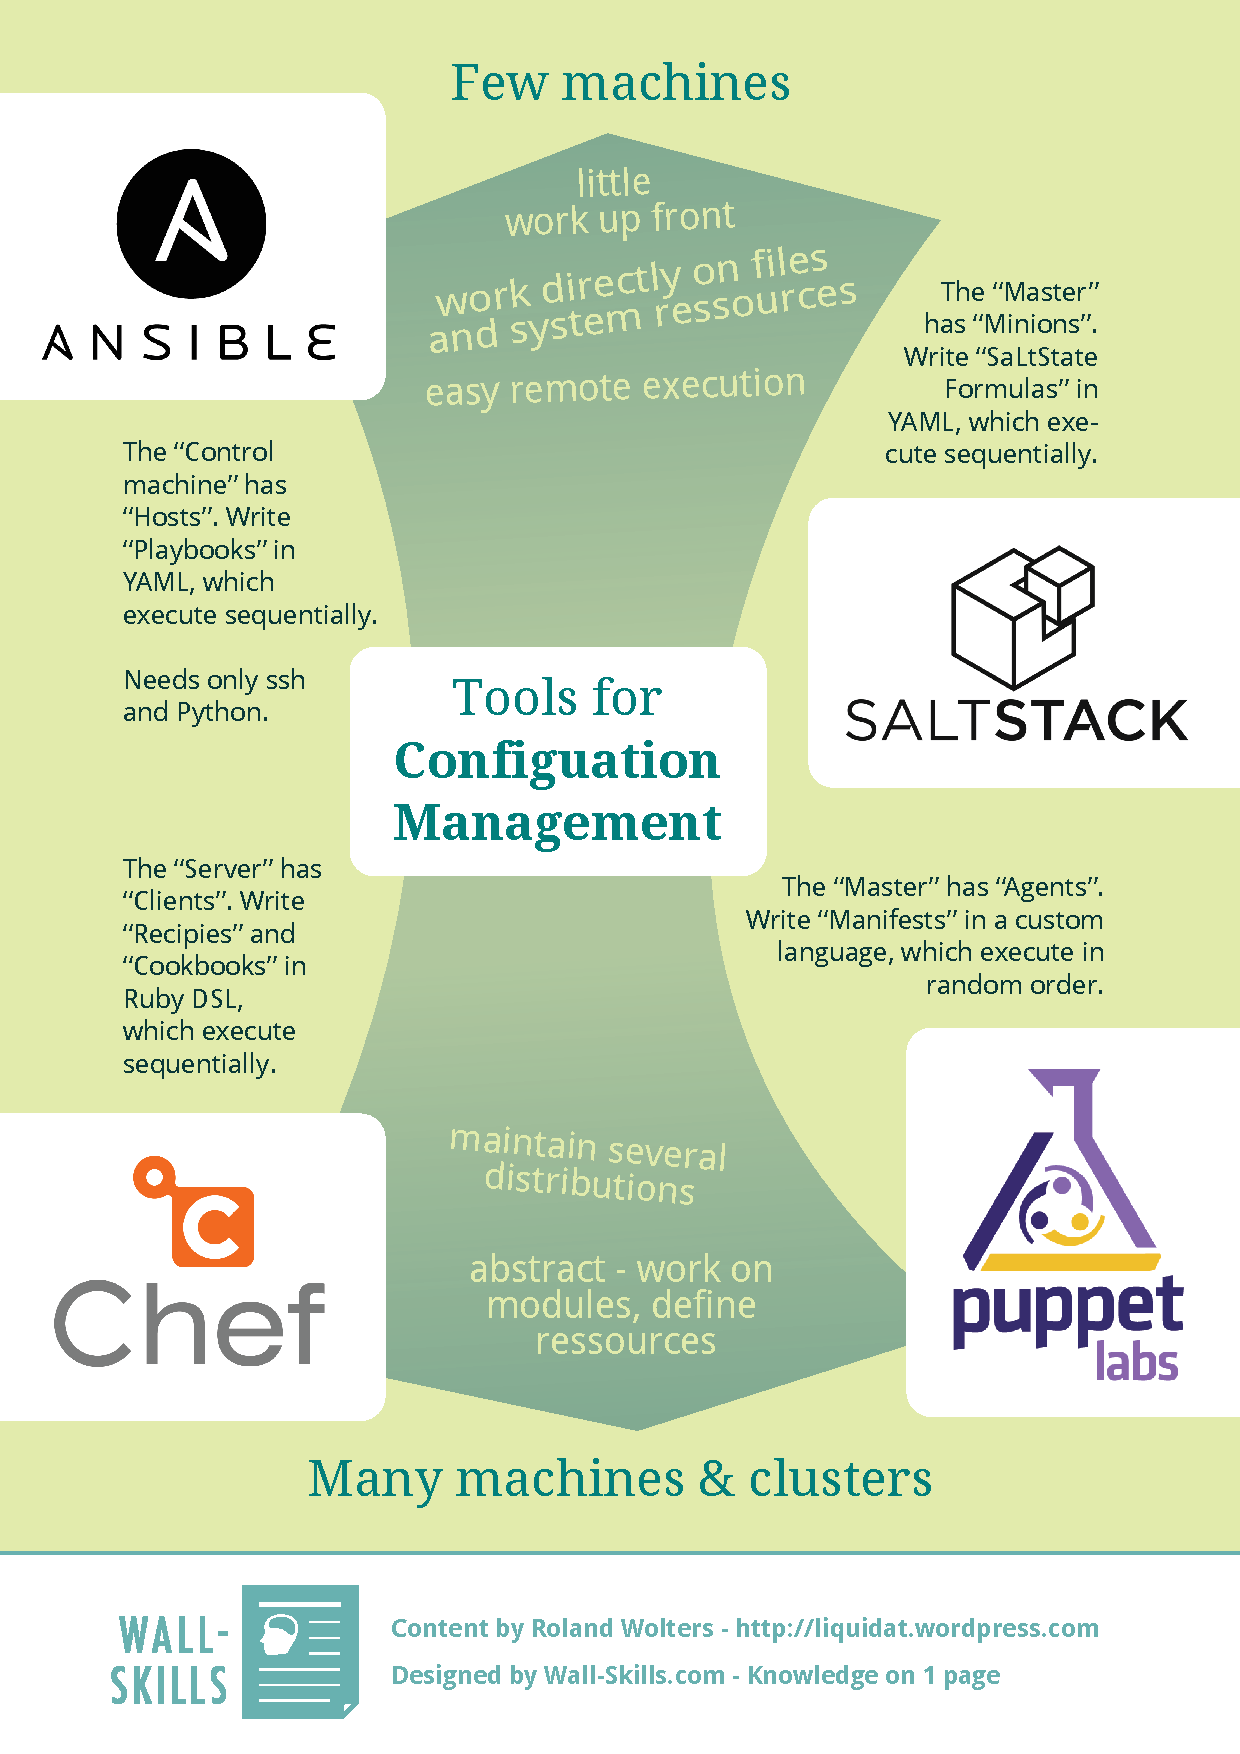
\includegraphics[height=1.0\textheight]{./images/compare.pdf}}
\end{center}
\end{frame}

%%%%%%%%%%%%
\begin{frame}
\bluetext{\href{http://www.intigua.com/blog/puppet-vs.-chef-vs.-ansible-vs.-saltstack}{\underline{http://www.intigua.com/blog/puppet-vs.-chef-vs.-ansible-vs.-saltstack}}}
\begin{center}
{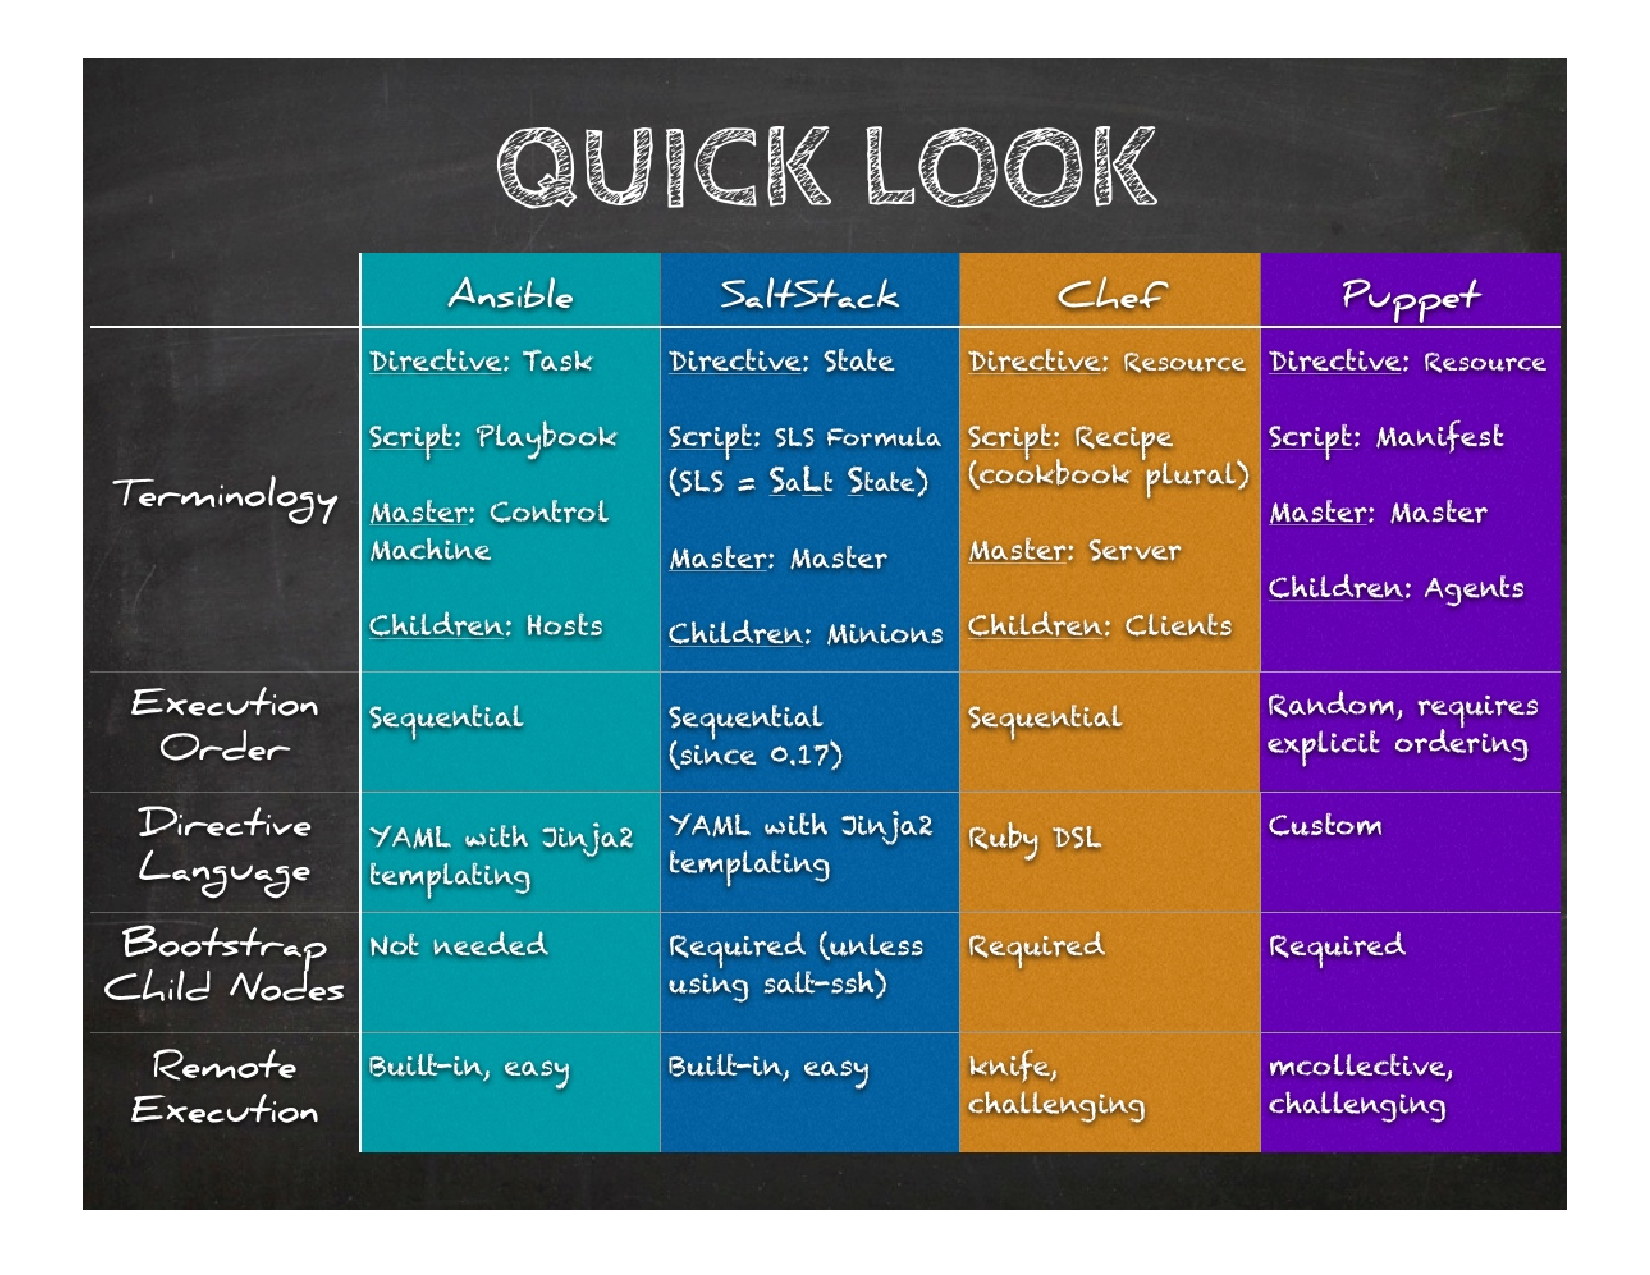
\includegraphics[height=1.0\textheight]{./images/compare2.pdf}}
\end{center}
\end{frame}

%%%%%%%%%%%%%%%%
\begin{frame}
\frametitle{Push-Based}

\hspace{1em}\bluetext{Chef and Puppet: ``pull-based'' by default:}
\vspace{0.8em}
%
\begin{enumerate}[\color{black}(1)]
\setlength\itemsep{0.7em}
%\addtolength{\itemindent}{1em}
\item You: make a change to a configuration management script.
\item You: push the change up to a configuration management central service.
\item Agent on server: wakes up after periodic timer fires.
\item Agent on server: connects to configuration management central service.
\item Agent on server: downloads new configuration management scripts.
\item Agent on server: executes configuration management scripts locally which change server state
\end{enumerate}

\vspace{2.4em}
\hspace{1em}\bluetext{Ansible is ``push-based'' by default:}
\vspace{0.8em}
 %
\begin{enumerate}[\color{black}(1)]
\setlength\itemsep{0.7em}
%\addtolength{\itemindent}{1em}
\item You: make a change to a playbook.
\item You: run the new playbook.
\item Ansible: connects to servers and executes modules, which changes server state.
\end{enumerate}

\end{frame}

%%%%%%%%%%%%%%%
\subsection{How to work with Ansible and how it works}
\begin{frame}[fragile, label=none]
%
\myinsertsubsection
\vspace{1em}

\begin{enumerate}[\color{black}(1)]
\setlength\itemsep{1.5em}
%\addtolength{\itemindent}{1em}
\item install Ansible:
\begin{Verbatim}[commandchars=\\\{\}]
\graytext{> pip install ansible}
\end{Verbatim}
\item write Ansible configurational file \texttt{\bf{ansible.cfg}}
\item write \texttt{\bf{hosts}} file with target machines to be configured
\item write a script called a {\it playbook} in Ansible, actually, a yaml-file
that defines final state of target machines
\item divide a playbook into ordered list of {\it tasks}
\item target machines ({\it hosts} or {\it remote servers}) to be configured are defined in playbook
\item run script:
\begin{Verbatim}[commandchars=\\\{\}]
\graytext{> ansible-playbook webservers.yml}
\end{Verbatim}
\end{enumerate}
\end{frame}

\begin{frame}[fragile]
%\begin{minipage}[t][5cm][b]{0,5\textwidth}
%\begin{minipage}[c][1em]{0,8\textwidth}
\begin{block}{Task:}
Configure three Fedora-based web servers to run nginx using Ansible.
\end{block}
\vspace{1em}
Call hosts as {\bf web1}, {\bf web2}, {\bf web3} and create a playbook with the tasks:
\begin{itemize}
\item Install nginx
\item Generate an nginx configuration file
\item Start the nginx service
\end{itemize}
\vspace*{2em}
{\bf Next step:}\\
\begin{Verbatim}[commandchars=\\\{\}]
\graytext{> ansible-playbook webservers.yml}
\end{Verbatim}
%\vspace{1em}
%{\bf What Ansible does:}
Ansible makes SSH connections to web1, web2, and web3.\\
\vspace{2em}
The first task looks like this:
\vspace{2em}
\begin{columns}[t]
\column{.4\textwidth}
%\hspace*{0.5cm}
\begin{beamercolorbox}[sep=-1.0em,rounded=true,shadow=true,center]{res1}
\begin{lstlisting}[language=yaml]
- name: Install nginx
  dnf: name=nginx
\end{lstlisting}
\end{beamercolorbox}
\end{columns}
\end{frame}


%%%%%%%%%%%%%%%%%%%%%%%%
\begin{frame}
\hspace{2em}\alert{Ansible will:}

\begin{enumerate}[\color{black}1.]
\addtolength{\itemindent}{1em}
\item Generate a Python script that installs the nginx package.
\item Copy the script to web1, web2, and web3.
\item Execute the script on web1, web2, web3.
\item Wait for the script to complete execution on all hosts.
\item Move to the next task.\\
.....
\end{enumerate}

%\vspace{1em}
\hspace{2em}\alert{How Anible works:}

\begin{itemize}
\item Ansible runs each task in parallel across all hosts.
\item Ansible waits until all hosts have completed a task before moving to the next task.
\item Ansible runs the tasks in the order that you specify them.
\item Ansible modules are {\it idempotent}.
\end{itemize}
\begin{center}
\vspace{-1.2em}
{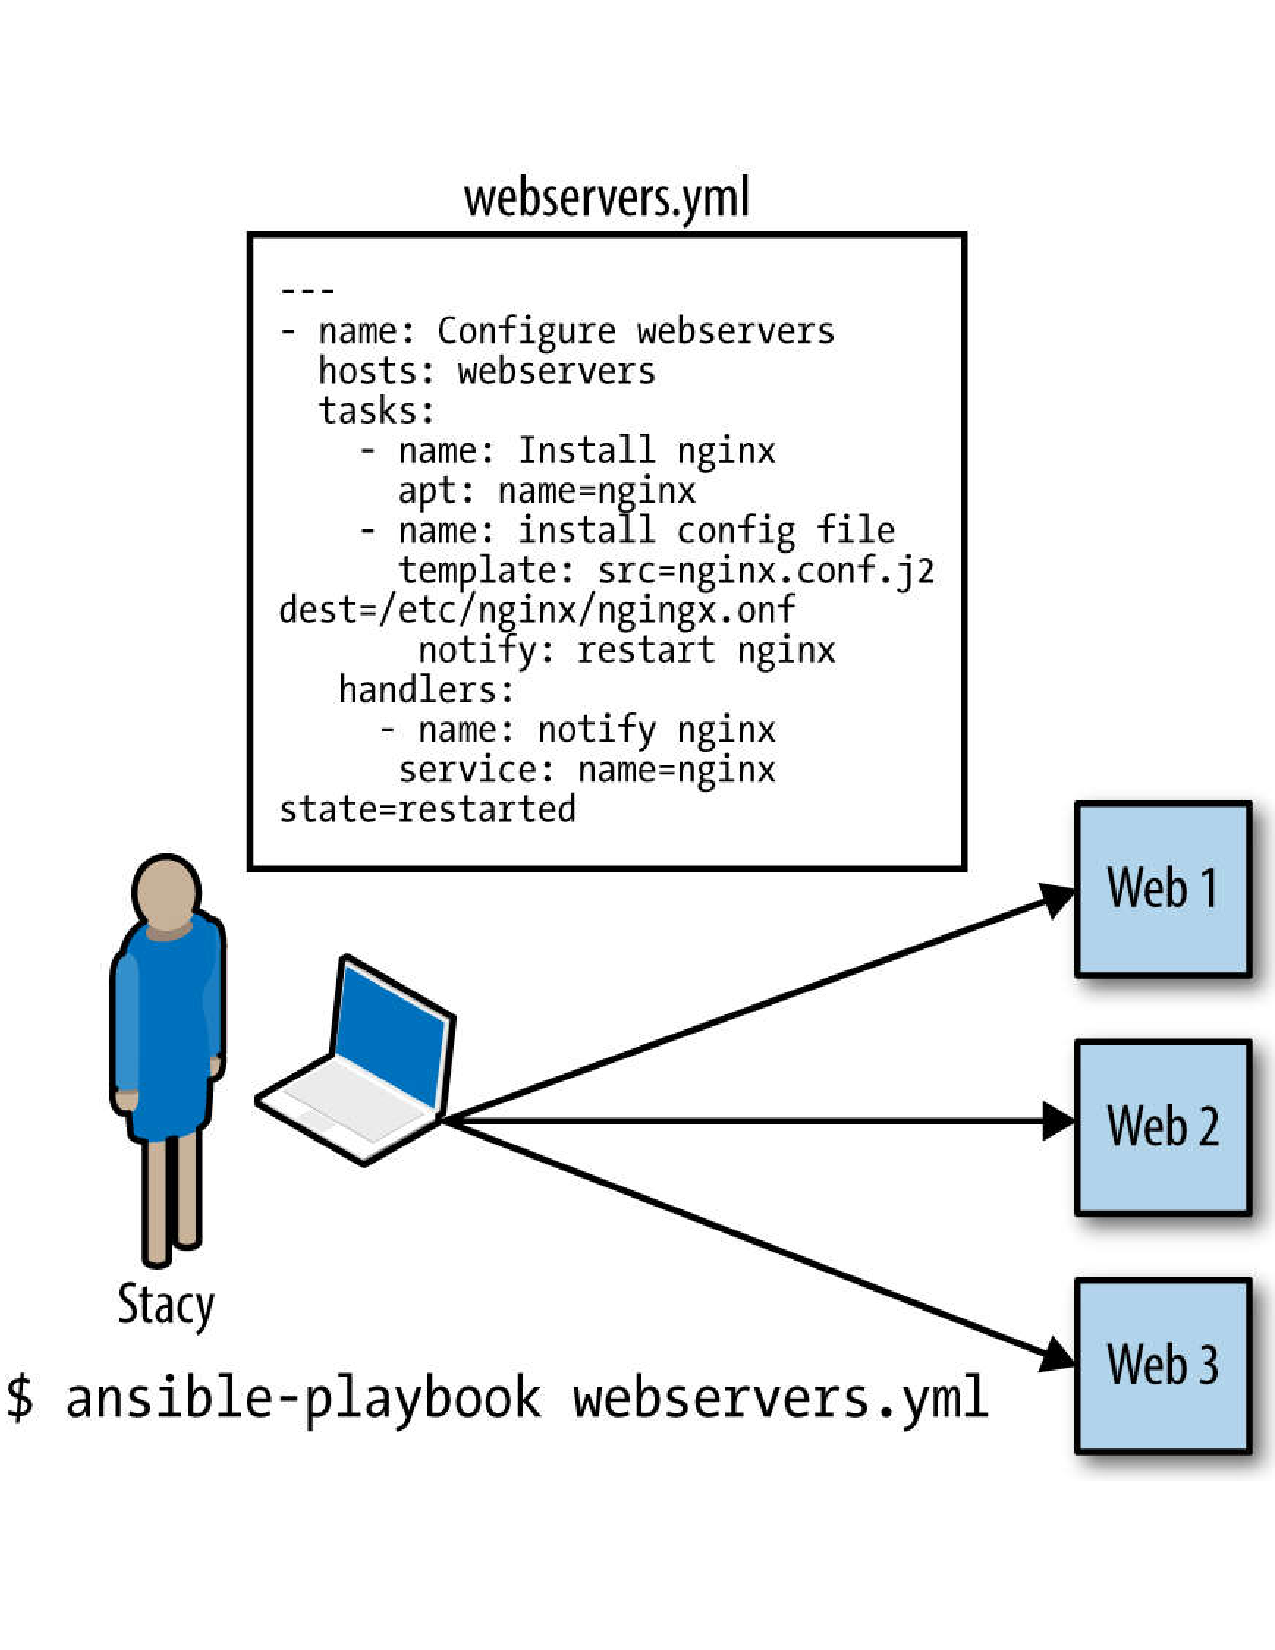
\includegraphics[width=0.32\textwidth]{./images/scheme.pdf}}
\end{center}

\end{frame}


%%%%%%%%%%%%%%%%%%%%%%%%%%%%%%%%%%%%%%%%%%%%%
\section{Anatomy of a Playbook}
\subsection{YAML Syntax}
\begin{frame}[fragile,label=yaml2]
\frametitlesection
\myinsertsubsection
\vspace{1em}
See: \bluetext{\small\href{http://docs.ansible.com/ansible/YAMLSyntax.html}{\underline{http://docs.ansible.com/ansible/YAMLSyntax.html}}}

\begin{columns}[t,onlytextwidth]
\column{.54\textwidth}
\begin{itemize}
  \item YAML: begins with \verb!---! and ends with \verb|...|
  \item List:
  \begin{beamercolorbox}[dp=1ex,left,leftskip=50ex,wd=0.9\textwidth,sep=-1.0em,rounded=true,shadow=true]{res1}
  \begin{lstlisting}[language=yaml]
---
# A list of fruits
fruits:
  - Apple
  - Orange
  - Strawberry
...
  \end{lstlisting}
  \end{beamercolorbox}

  \item Dictionary
  \begin{beamercolorbox}[wd=0.9\textwidth,sep=-1.0em,rounded=true,shadow=true,center]{res1}
  \begin{lstlisting}[language=yaml]
# An employee record
volodya:
  name:  Volodya Maksymiv
  job:   Developer
  skill: Elite
  \end{lstlisting}
  \end{beamercolorbox}
\end{itemize}
\end{columns}
\end{frame}

\begin{frame}[fragile,label=yaml3]
\begin{columns}[t,onlytextwidth]
\column{1.\textwidth}
\begin{itemize}
\item List and Dictionary abbreviated form
  \begin{beamercolorbox}[wd=0.9\textwidth,sep=-1.0em,rounded=true,shadow=true,center]{res1}
  \begin{lstlisting}[language=yaml]
---
volodya: {name: V. Maksymiv, job: Developer, skill: Elite}
fruits: ["Apple", "Orange", "Strawberry", "Mango"]
  \end{lstlisting}
  \end{beamercolorbox}

\item Boolean
  \begin{beamercolorbox}[wd=0.9\textwidth,sep=-1.0em,rounded=true,shadow=true,center]{res1}
  \begin{lstlisting}[language=yaml]
create_key: yes
needs_agent: no
knows_oop: True
likes_emacs: TRUE
uses_cvs: false
  \end{lstlisting}
  \end{beamercolorbox}

\item Spanning multiple lines
  \begin{beamercolorbox}[wd=0.9\textwidth,sep=-1.0em,rounded=true,shadow=true,center]{res1}
  \begin{lstlisting}[language=yaml]
include_newlines: |
  exactly as you see
  will appear these three
  lines of text

ignore_newlines: >
  this is really a
  single line of text
  despite appearances
  \end{lstlisting}
  \end{beamercolorbox}

\end{itemize}

\end{columns}

\end{frame}
%%%%%%%%%%%%%%%%%%%%%%%%%%%%%%%%%%%%%%%%%%%%%%%%%%%%%%%%%%%%%%%%%%%%%%%%%%%%%%%%%%%%%%%%%%%%%%


\begin{frame}[fragile,label=yaml4]
\begin{columns}[t,onlytextwidth]
\column{1.\textwidth}
\begin{itemize}
\item Use double quotes if string contains a colon
  \begin{beamercolorbox}[wd=0.9\textwidth,sep=-1.0em,rounded=true,shadow=true,center]{res1}
  \begin{lstlisting}[language=yaml]
foo: if you want to put colon: here (wrong)
foo2: if you want to put colon:here (correct)
foo3: "if you want to put colon: here (correct)"
  \end{lstlisting}
  \end{beamercolorbox}

\item Use double quotes if you have a variable
  \begin{beamercolorbox}[wd=0.9\textwidth,sep=-1.0em,rounded=true,shadow=true,center]{res1}
  \begin{lstlisting}[language=yaml]
foo: "{{ variable }}"
foo2: "{{ variable }}/additional/string/literal"
  \end{lstlisting}
  \end{beamercolorbox}

\end{itemize}

\end{columns}

\end{frame}

%%%%%%%%%%%%%%%%%%%%%%%%%%%%%%%%%%%%%%%%%%%%%%%%%%%%%%%%%%%%%%%%%%%%%%%%%%%%%%%%%%%%%%%%%%%%%%
%%%%%%%%%%%%%%%%%%%%%%%%%%%%%%%%%%%%%%%%%%%%%%%%%%%%%%%%%%%%%%%%%%
\subsection{Playbook example (webservers.yml)}
\begin{frame}[fragile, label=none]
%
\myinsertsubsection
%
%\myinsertsubsection
%\vspace{2mm}
%{\bf Simple playbook} (webservers.yml):
%\vspace{1mm}
%
%\begin{center}
%\begin{columns}[t,onlytextwidth]
\begin{columns}[t]
\column{1.0\textwidth}
%\hspace*{0.5cm}
\begin{beamercolorbox}[sep=-1.0em,rounded=true,shadow=true,center]{res1}
\begin{lstlisting}[language=yaml]
---
- name: Configure webservers with nginx
  hosts: webservers
  become: yes
  vars:
    conf_file: /etc/nginx/sites-available/default

  tasks:
    - name: Install nginx
      dnf: name=nginx

    - name: Copy nginx config file
      template: "src=templates/nginx.conf.j2 dest={{ conf_file }}"

    - name: restart nginx
      service: name=nginx state=restarted
\end{lstlisting}
\end{beamercolorbox}
\end{columns}
\vspace{2em}
\bluetext{List of main playbook components:}
\begin{columns}[c,onlytextwidth]
\column{.40\textwidth}
\begin{itemize}
\item play
\item hosts
\item user running the script
\end{itemize}
\column{.40\textwidth}
\begin{itemize}
\item vars
\item task
\item module
\end{itemize}
\end{columns}
%

%\end{center}
\end{frame}
%%%%%%%%%%%%%%%%%%%%%%%%%%%%%%%%%%%%%%%%%%%%%%%%%
\section{Work with Vagrant}
\subsection{Spinning up virtual machine}
\begin{frame}[fragile]
\frametitlesection
\myinsertsubsection
\vspace{1em}
Create virtual machine:
\begin{Verbatim}[commandchars=\\\{\}]
\graytext{> vagrant init fedora/25-cloud-base}
\graytext{> vagrant up}
\end{Verbatim}

\vspace{1em}
Login with SSH:
\begin{Verbatim}[commandchars=\\\{\}]
\graytext{> vagrant ssh}
\end{Verbatim}

\vspace{1em}
See ssh configuration of Vagrant (exit from virtual machine first):
\begin{Verbatim}[commandchars=\\\{\}]
\graytext{> vagrant ssh-config}
\end{Verbatim}

\begin{beamercolorbox}[sep=-0.5em,rounded=true,shadow=true,center]{res1}
\small
\begin{Verbatim}[commandchars=\\\{\}]
Host default
  HostName 127.0.0.1
  User vagrant
  Port 2222
  UserKnownHostsFile /dev/null
  StrictHostKeyChecking no
  PasswordAuthentication no
  IdentityFile /Users/v.maksymiv/ansiblebook/.vagrant/machines/default/virtualbox/private\_key
  IdentitiesOnly yes
  LogLevel FATAL
\end{Verbatim}
\end{beamercolorbox}
\end{frame}
%%%%%%%%%%%%%%%%%%%%%%%%%%%%%%%%%%%%%%%%%%%%%%%%%
\subsection{Check Ansible connection to VM}
\begin{frame}[fragile]
\myinsertsubsection

\vspace{1.5em}
Perform manual SSH login:
\begin{Verbatim}[commandchars=\\\{\}]
\graytext{> ssh vagrant@127.0.0.1 -p 2222 -i /Users/v.maksymiv/ansiblebook/playbooks/}
\graytext{.vagrant/machines/default/virtualbox/private_key}
\end{Verbatim}
\vspace{1.5em}
Create the \verb|playbooks/hosts| file:

\hspace{1em}
\begin{beamercolorbox}[wd=0.85\textwidth,sep=-0.5em,rounded=true,shadow=true,center]{res1}
\small
\begin{Verbatim}
testserver     ansible_ssh_host=127.0.0.1 ansible_ssh_port=2222 \
ansible_ssh_user=vagrant \
ansible_ssh_private_key_file=.vagrant/machines/default/virtualbox/private_key
\end{Verbatim}
\end{beamercolorbox}

\vspace{1.5em}
\normalsize
Check Ansible connection with the virtual machine:
\begin{Verbatim}[commandchars=\\\{\}]
\graytext{> ansible testserver -i hosts -m ping}
\end{Verbatim}

\hspace{1em}
\begin{beamercolorbox}[wd=0.32\textwidth,sep=-0.5em,rounded=true,shadow=true,center]{res1}
\small
\begin{Verbatim}
testserver | success >> {
"changed": false,
"ping": "pong"
}
\end{Verbatim}
\end{beamercolorbox}

\vspace{1.5em}
\normalsize
Debug if something goes wrong:
\begin{Verbatim}[commandchars=\\\{\}]
\graytext{> ansible testserver -i hosts -m ping -vvvv}
\end{Verbatim}
\end{frame}
%%%%%%%%%%%%%%%%%%%%%%%%%%%%%%%%%%%%%%%%%%%%%%%%%%%%%%%%%%%%%%%%%%%%%%%%%%%%%
%\subsection{Inventory Generated by Vagrant}
%\begin{frame}[fragile]
%\frametitlesubsection
%When Vagrant runs, it generates an Ansible inventory file named
%
%\vspace{1em}
%\verb|.vagrant/provisioners/ansible/inventory/vagrant_ansible_inventory|
%
%# Generated by Vagrant
%
%default ansible_ssh_host=127.0.0.1 ansible_ssh_port=2222 ansible_ssh_user='vagrant' ansible_ssh_private_key_file='/x/.vagrant/machines/default/virtualbox/private_key'
%
%
%\end{frame}
%%%%%%%%%%%%%%%%%%%%%%%%%%%%%%%%%%%%%%%%%%%%%%%%%%%%%%%%%%%%%%%%%%%%%%%%%%%%
\renewcommand\Switchsubsection{0}
\section{ansible.cfg file usage }
\begin{frame}[fragile]
\frametitlesection
Create \verb|playbooks/ansible.cfg| file:

\hspace{1em}
%\begin{Verbatim}
\begin{beamercolorbox}[wd=0.75\textwidth,sep=-0.5em,rounded=true,shadow=true,center]{res1}
\begin{lstlisting}[language=conf]
[defaults]
hostfile = hosts
remote_user = vagrant
private_key_file = .vagrant/machines/default/virtualbox/private_key
host_key_checking = False
\end{lstlisting}
\end{beamercolorbox}
%\end{Verbatim}

\vspace{2em}
Now \verb|hosts| file can be reduced to:

\hspace{1em}
\begin{beamercolorbox}[wd=0.75\textwidth,sep=-0.5em,rounded=true,shadow=true,center]{res1}
\small
\begin{Verbatim}
testserver     ansible_ssh_host=127.0.0.1  ansible_ssh_port=2222
\end{Verbatim}
\end{beamercolorbox}

\vspace{1.5em}
\normalsize
Check Ansible connection with the virtual machine again:
\begin{Verbatim}[commandchars=\\\{\}]
\graytext{> ansible testserver -i hosts -m ping}
\end{Verbatim}

\vspace{1em}
Running arbitrary command:
\begin{Verbatim}[commandchars=\\\{\}]
\graytext{> ansible testserver -m command -a "ps aux"}
\end{Verbatim}

\vspace{1em}
Running arbitrary command as a root:
\begin{Verbatim}[commandchars=\\\{\}]
\graytext{> ansible testserver -s -m command -a "tail /var/log/syslog"}
\end{Verbatim}
\end{frame}
%%%%%%%%%%%%%%%%%%%%%%%%%%%%%%%%%%%%%%%%%%%%%%%%%%%%%%%%%%%%%%%%%%%%%%%%%%%%
%++++++++++++++++++++++++++++++++++++++++
\begin{frame}[plain,c,label=thanks]
\begin{center}
\textrm{\bluetext{\Large THANK YOU!}}
\end{center}
\end{frame}
\end{document}
